\documentclass[12pt]{beamer}

\usepackage[utf8]{inputenc}
\usepackage{graphicx}
\usepackage{amsmath}
\usepackage{color}
\DeclareGraphicsRule{*}{mps}{*}{}

\newcommand{\javakeyword}[1]{\textcolor{violet}{\texttt{{#1}}}}

\usetheme{Rochester}

\title{Objektorientiertes Design: Grundlagen}
\author{Kilian Gärtner, Rosario Raulin}
\date{Wintersemester 2012/13}

\begin{document}

\frame{\titlepage}

\begin{frame}
	\frametitle{Agenda}
	\tableofcontents
\end{frame}

\section{Abstrakte Basisklasse}
\begin{frame}
	\frametitle{(Abstrakte) Basisklassen}
	
	\begin{itemize}
		\item Basisklasse: gemeinsames Verhalten von Subklassen zentral definiert
		\item abstrakt: Basisklasse so allgemein, dass bestimmte Bestandteile nicht
		sinnvoll definiert werden können
		\item Schlüsselwort \javakeyword{abstract} in Java (vor Klassen und Methoden)
		\item keine konkreten Objekte (mit \javakeyword{new}) erzeugbar
	\end{itemize}
\end{frame}

\begin{frame}
	\frametitle{Beispiel: Geometrische Objekte}
	\centerline{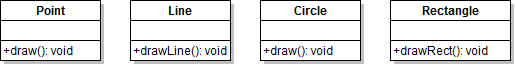
\includegraphics[scale=0.6]{src/img/Figures}}
\end{frame}

\begin{frame}
	\frametitle{Besser: Abstrakte Basisklasse}
	\centerline{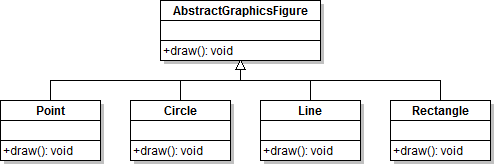
\includegraphics[scale=0.6]{src/img/AbstractGraphicsFigure}}
\end{frame}

\begin{frame}
	\frametitle{Vor- und Nachteile}
	\textbf{Abstrakte Basisklasse}
	\newline
	\begin{itemize}
		\item[+] einheitliche, modulare Implementierung
		\item[+] erweiterbar
		\item[+] keine Coderedundanz
		\item[-] "Explosion" der Klassenhierarchie möglich
	\end{itemize}
\end{frame}

\begin{frame}
	\frametitle{Beispiel: Explosion der Klassenhierarchie}
	\centerline{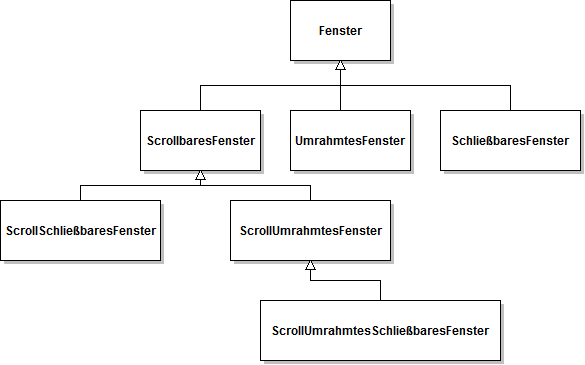
\includegraphics[scale=0.5]{src/img/Fenster}}
\end{frame}

\section{Interfaces}

\begin{frame}
	\frametitle{Interfaces}
	\begin{itemize}
		\item Vertrag zwischen aufrufender und implementierender Klasse
		\item eine Klasse muss Interface-Methoden implementieren
		\item wir entkoppeln Realisierung und Spezifikation
		\item "can-act-like"-Beziehung (Rolle)
	\end{itemize}
\end{frame}

\begin{frame}
	\frametitle{Beispiel: Comparable}

	\centerline{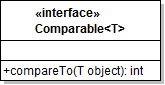
\includegraphics[scale=0.5]{src/img/Comparable}}
	\vspace{5mm}
	\begin{itemize}
		\item dient dem Vergleich zweier Objekte einer Klasse
		\item beschreibt eine (transitive) Relation:
			\begin{itemize}
				\item \texttt{x.compareTo(y) > 0 \(\Leftrightarrow\) x > y}
				\item \texttt{x.compareTo(y) = 0 \(\Leftrightarrow\) x = y}
				\item \texttt{x.compareTo(y) < 0 \(\Leftrightarrow\) x < y}
			\end{itemize}
	\end{itemize}
\end{frame}

\begin{frame}
	\frametitle{Vor- und Nachteile}
	\textbf{Interfaces}
	\newline
	\begin{itemize}
		\item[+] Entkoppelung von Spezifikation und Realisierung
		\item[+] Modularität
		\item[+] zentrale Definition öffentlich erreichbarer Funktionen
		\item[+] Java: beliebig viele Interfaces pro Klasse
		\item[-] keine Konstruktoren
		\item[-] nur \texttt{public}-Methoden
	\end{itemize}
\end{frame}

\section{Kombination von Basisklassen und Interfaces}

\begin{frame}
	\frametitle{Kombination beider Ansätze}
	\centerline{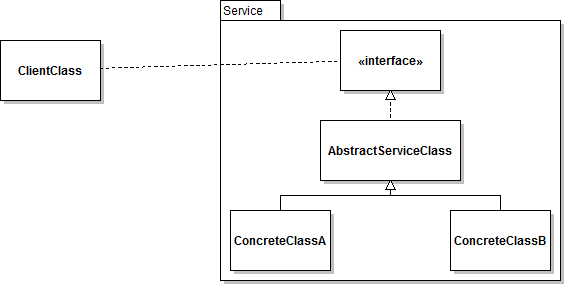
\includegraphics[scale=0.5]{src/img/Kombi}}
\end{frame}

\begin{frame}
	\frametitle{Vorteile der Kombination}
	Wir erhalten damit die Vorzüge beider Ansätze:
	\begin{itemize}
		\item[+] Modularität
		\item[+] Basisfunktionalität und Spezialisierung
		\item[+] wenig/keine Redundanz
		\item[o] ein wenig mehr Implementierungsaufwand
	\end{itemize}
\end{frame}

\section{Beispiele aus der Praxis}

\begin{frame}
	\frametitle{Live-Demo}
	\vspace*{\fill}
		\centerline{\huge Beispiele aus der Praxis}
	\vspace*{\fill}
\end{frame}

\begin{frame}
	\frametitle{Fragen und Antworten}
	\vspace*{\fill}
		\centerline{\large Gibt es noch Fragen?}
	\vspace*{\fill}
		\pause
		\centerline{\large Vielen Dank für Eure Aufmerksamkeit!}
	\vspace*{\fill}
\end{frame}

\section{Übungsaufgabe}

\begin{frame}
	\frametitle{Nun zum praktischen Teil...}
	\begin{enumerate}
		\item Modelliere eine Klassenhierarchie für Lebensmittel! Versuche auch das
		Konzept der abstrakten Basisklasse zu verwenden!
		\item Implementiere die Hierarchie bis zur 2. oder 3. Ebene!
		\item Suche dir eine konkrete Klasse heraus. Implementiere Comparable und
		teste deine Implementierung!
		\item ...
	\end{enumerate}
\end{frame}

\begin{frame}
	\frametitle{Peelable}
	\centerline{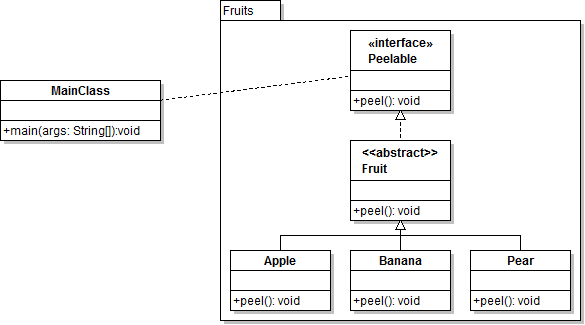
\includegraphics[scale=0.5]{src/img/Fruits}}
\end{frame}

\end{document}

